\documentclass[paper=a4,11pt,titlepage,twoside=true,headings=normal,numbers=noenddot,captions=tableabove,listof=totoc,index=totoc,bibliography=totoc, ngerman]{scrreprt}
%-----------------------------------------------------------------
\usepackage{etoolbox}
\newbool{deutsch}
\booltrue{deutsch}	% comment out to switch document to english
%-----------------------------------------------------------------
%\usepackage{amsmath} % abgesetzte Formeln zentriert in der Zeile
%\usepackage[fleqn,intlimits]{amsmath} % [fleqn] abgesetzte Formeln mit festem Abstand zum linken Rand
\usepackage{microtype}
\usepackage[reqno,intlimits]{amsmath} % [reqno] um die gleichungsnummerierung rechts zu haben
% intlimits: Grenzen für Integrale unterhalb und oberhalb des Zeichens
\usepackage{amssymb}
\usepackage{array}
\ifbool{deutsch}{%
    \usepackage[ngerman]{babel}
}{%
    \usepackage[english]{babel}
}
\usepackage{varioref}
\usepackage[T1]{fontenc}
\usepackage[utf8]{inputenc}
%---------------------------
\usepackage{booktabs}
\usepackage{calc}
\usepackage{cancel}
\usepackage[labelfont={footnotesize,sf,bf},textfont={footnotesize,sf}]{caption} %Format (Textgröße, Textform) für Bildtext 
%normalsize
%scriptsize
% sc --> smallcaps
% bf --> bold face
% sf --> sans serif
\usepackage[table]{xcolor}
\usepackage[right]{eurosym}
\usepackage{ellipsis}
\usepackage{graphicx}
\usepackage{float}
%----------------------------------------
\usepackage{gensymb}
\usepackage{csquotes}
\usepackage{listings}
\usepackage{longtable}
\usepackage{lastpage}
\usepackage{lscape}
\usepackage{lmodern} %-- Silbentrennung
\usepackage{makeidx}
\usepackage{multirow}
\usepackage{multicol}
%\usepackage[intoc]{nomencl}   % zwei Spalten beim Formelzeichenverzeichnis
\usepackage[intoc]{nomentbl} %vier Spalten bei Formelzeichenverzeichnis
\usepackage{nicefrac}
\usepackage{paralist}
\usepackage{parallel}
\usepackage{pdfpages} % https://www.ctan.org/pkg/pdfpages
% Define user colors using the RGB model
%\usepackage{colortbl}
%\definecolor{dunkelgrau}{rgb}{0.8,0.8,0.8}
%\definecolor{hellgrau}{rgb}{0.95,0.95,0.95}
%\usepackage{pgfplots}
\usepackage[figuresright]{rotating}
\usepackage{scrlayer-scrpage}
\usepackage[locale=DE,per-mode=symbol,range-units = repeat,separate-uncertainty=true]{siunitx} %nicht zusammen mit sistyle %---------
\DeclareSIUnit{\amperehour}{Ah}
\DeclareSIUnit{\watthour}{Wh}
% \usepackage[font={scriptsize,sl},captionskip=3pt]{subfig} % für die Unterbilder %---------
\usepackage{subcaption}
\usepackage{shortvrb}
\usepackage{tablefootnote}
\usepackage{tabularx}
\usepackage{tabulary}
\usepackage{textcomp}
\usepackage{tocbasic}
% \usepackage{tikz}
\usepackage{times}
\usepackage{units}
\usepackage{xurl}
\usepackage{wrapfig}
\usepackage{xr-hyper}
\usepackage{arydshln} %für \hdashline[5pt/2pt] % muss am Ende stehen, sonst gibt es Probleme mit xcolor
\usepackage{hyperref}
\hypersetup{
    colorlinks=true, % Color links instead of disgusting boxes :barfing_emoji:
    linkcolor={black}, % Color of internal links
    citecolor={black}, % Color of citations
    urlcolor={blue} % Color of external hyperlinks
}
%\usepackage{unicode-math}
%\usepackage[toc,symbols]{glossaries} %---------- muss nach hyperref stehen
\usepackage[nonumberlist, acronym, toc, section]{glossaries} % muss nach hypersetup stehen
%----------------
%\usepackage{romannum} % Seitenzahlen in römischen Ziffern
\usepackage{scrhack}
\usepackage[style=numeric, citestyle=numeric, backend=biber, date=short]{biblatex}
\usepackage[useregional]{datetime2}
\usepackage{cleveref}
% \usepackage{isotope} % um chemische gleichungen hübscher darstellen zu können
% \usepackage{framed} % rahmen um dinge malen können
\usepackage[inkscapearea=page]{svg} % um auch vektorgrafiken als bild einfügen zu können https://ctan.org/pkg/svg
% \usepackage{adjustbox} % skaliert floats dynamischer (anti-over/underfull)
\usepackage[numbered]{bookmark} % platziert im pdf reader bei der kapitelübersicht die jeweiligen kapitelnummer vor die kapitelüberschriften
% ---------- Make floats stay within the chapter/section/subsection they got placed ------------------
\usepackage{placeins}
\let\Oldsection\section
\renewcommand{\section}[1]{\FloatBarrier\Oldsection{#1}}
\let\Oldsubsection\subsection
\renewcommand{\subsection}[1]{\FloatBarrier\Oldsubsection{#1}}
\let\Oldsubsubsection\subsubsection
\renewcommand{\subsubsection}[1]{\FloatBarrier\Oldsubsubsection{#1}}
%===================== define VARIABLES ==========================
% --------------------- Names ------------------------------------
\newcommand{\thefirstnameA}{Dennis}
\newcommand{\thelastnameA}{Hunter}
\newcommand{\thefirstnameB}{Dung}
\newcommand{\thelastnameB}{Pie}
\newcommand{\thefirstnameC}{Donkey}
\newcommand{\thelastnameC}{Shorts}
% --------------------- Titel Course -----------------------------
\newcommand{\titleLV}{Projektarbeit}
%---------------------- Document Titel ---------------------------
\newcommand{\subtitleA}{Konzeption und Realisierung eines Antriebssystems für ein elektrisches Longboard}
\newcommand{\subtitleB}{``MotherBoard''}
%-------------- Deprecated below but still usable ----------------
%---------------------- Dates ------------------------------------
% \newcommand{\versuch}{2} % Versuchsnummer einfügen
% \newcommand{\dateLV}{17.11.2020} % Datum einfügen
% \newcommand{\deadline}{28.02.2022} % Abgabedatum ist der 1.12.2020
% \newcommand{\dateLVa}{December 1st, 2020}
% \newcommand{\dateLVb}{December 8th, 2020}
%:::::::::::::::::::::::::::::::::::::::::::::::::::::::::::::::::
\input{pre-page-layout}
\input{pre-header-footer-2010}
\input{pre-header-footer-text-report}
\input{pre-nomenclature-layout}
% \input{pre-other-layouts}
\DeclareNameAlias{author}{family-given}
\DeclareNameAlias{editor}{family-given}
\DeclareNameAlias{translator}{family-given}
\addbibresource{literature.bib}
%------DEBUGGING--------------------------------------------------
% \usepackage[showframe]{geometry} % comment out for live version
% \usepackage{layout}
% \usepackage{showframe}
% \usepackage[export]{adjustbox} % adds aside others the <frame> option to \includegraphics[]{}. this makes there borders visible and helps debugging/aligning
%-----------------------------------------------------------------
\begin{document}
%-----------------------------------------------------------------
\input{chapters/0_top}
\pagenumbering{Roman}
\tableofcontents
\newpage
\printnomenclature[5cm]
% \addchap{Nomenklatur}
    \begin{table}[h]
        \begin{tabular}{@{}ll@{}}%
            \(a\) & A letter\\
            & \\
            \(\alpha\) & Greek jibberish\\
    \end{tabular}\label{tab:Nomenclature}
    \end{table}

\addchap{Abkürzungen}
    \begin{table}[h]
        \begin{tabular}{@{}ll@{}}%
            BLDC & Brushless Direct Current \\
            ESC & Electronic Speed Controller\\
            PEV & Persönliches elektrisches Vehikel\\
            PEKV & Persönliches elektrisches Kleinstvehikel\\
            ePKW & Elektrischer Personenkraftwagen\\
            & \\
            & \\
    \end{tabular}\label{tab:acronyms}
    \end{table}
%-----------------------------------------------------------------
\clearpage\pagenumbering{arabic}
% LTeX: language=de-DE
\chapter{Einleitung}
	%
	Weltweit findet derzeit auf politischer wie gesellschaftlicher Ebene ein Umdenken im Transportwesen statt --~sei es der Transport von Gütern, Fahrgästen oder im Individualverkehr.
	Angefeuert durch den unmittelbaren monetären Druck durch steigende Treibstoffpreise, die immer deutlicher werdenden Folgen fortdauernder CO\textsubscript{2}-Emissionen aber auch Lebensqualität beeinflussende Faktoren wie Staus und abnehmende Luftqualität in urbanen Gebieten treibt eine wachsende Zahl Menschen aus Auto heraus auf alternative Transportmöglichkeiten.
	Neben der klassischen Möglichkeit des Fahrrades kam mit erheblichen Verbesserungen und der deutlich breiteren Verfügbarkeit der Lithiumbatterie-Technologie ein Wandel des gesellschaftlichen Lebens einher, wie es vergleichbar zuletzt geschah, als das Smartphone die Bühne der Welt betrat -~die Elektrifizierung des Individualverkehrs.
	Nachdem einige Vorreiterstädte bereits früh mit baulichen Maßnahmen etwa durch Herabsetzen innerörtlicher Geschwindigkeitsbegrenzungen, Ausbau von Fahrradwegen oder Zuwachs öffentlicher Verkehrsmittel reagierten, ziehen nun immer mehr Städte nach.
	Dieser wechselseitige Trend bildet sich auch in der politischen Stimmung ab mit einer der wichtigsten Novellen für das öffentliche Verkehrsbild, die die ``\textit{Verordnung über die Teilnahme von Elektrokleinstfahrzeugen am Straßenverkehr und zur Änderung weiterer straßenverkehrsrechtlicher Vorschriften}'' von 2019 mit sich zog~\cite{Bundesgesetzblatt.2019}.
	Sie leutete den Advent breit verfügbarer persönlicher elektrischer Kleinstvehikel (PEKV)\nomenclature[A]{PEKV}{Persönliche elektrische Kleinstvehikel} zur Überbrückung der ``letzten Meile'' ein.\par\medskip
	%
	Die Kategorie elektrifizierter persönlicher Fahrzeuge lässt sich grob unterteilen in elektrische Personenkraftwagen (ePKW)\nomenclature[A]{ePKW}{Elektrische Personenkraftwagen}, persönliche elektrische Vehikel (PEV)\nomenclature[A]{PEV}{Persönliche elektrische Vehikel} und --~wie oben bereits erwähnt~-- die persönlichen elektrischen Kleinstvehikel in der kleinsten Variante.
	Zwar dominiert die erste Gruppe gegenwärtige politische Bemühungen zum Thema, gerade im städtischen Raum bieten sie jedoch kaum bis kein Potenzial, Infarkte des Straßenverkehrs zu vermeiden.
	Die Ladeinfrastruktur ist noch nicht einheitlich und flächendeckend geregelt und allem voran sind sie preislich für breite Teile der Bevölkerung unattraktiv.
	Vielversprechender sind Vertreter der beiden letztgenannten Gruppen.
	Dem Statistischen Bundesamt zufolge besaßen zu Jahresanfang~2020 etwa jeder neunte deutsche Haushalt oder \SI{11,4}{\percent} zumindest ein elektrisch angetriebenes Fahrrad.
	Während sie Anfang 2015 mit \(\sim \SI{4}{\percent}\) noch in etwa jedem 25. Haushalt aufzufinden waren kann hier eine Verbreitung um fast das Dreifache verzeichnet werden~\cite{zahl.der.ebikes.StatistischesBundesamt.2020.09.28}.\par\medskip
% LTeX: language=de-DE
\chapter{Konzeption}\label{sec:conception}
% ===============================================
% Nomenclatures
% ===============================================
\nomenclature[A]{ABS}{Acrylnitrilbutadienstyrol}%
\nomenclature[A]{BS}{Board Side}%
\nomenclature[A]{RS}{Road Side}%
\nomenclature[A]{ESC}{Elektronischer Speed Controller}%
\nomenclature[A]{BLDC}{Brushless Direct Current}%
%
	Um Konsistenz mit Literatur und Marktrecherchen sicherzustellen werden im Rahmen dieser Arbeit technische Begriffe aus dem Skater-Jargon genutzt.
	% Während Skateboarding einerseits keinesfalls als neuartiges Phänomen zu bezeichnen ist und andererseits in den vergangenen fünf Jahren eine Renaissance erlebt hat, kann, gerade im nicht-englischsprachigen Raum, nicht davon ausgegangen werden, dass alle Lesenden mit der Terminologie vertraut sind.
	Zu einigen Komponenten existieren keine definierte deutschsprachigen Begriffe.
	Daher wird im Folgenden zunächst Fokus auf eine Begriffskonvention gelegt und in diesem Rahmen funktionale Kernkomponenten eines Skate- bzw. Longboards\footnote{\hspace{1mm} Baulich zwar leicht zu unterscheiden, jedoch aus den gleichen Kernkomponenten und -funktionalitäten aufgebaut.} erläutert.
	Freie Übersetzungen des Autors sind kursiv und befinden sich in Klammer.\par\medskip
	%
	Das Antriebssystem soll in ein vorgegebenes, übergeordnetes System bestehend aus mechanischen und elektronischen Komponenten eingebettet werden.
	Sowohl das übergeordnete System, als auch die Einsatzumgebung definieren konstruktive Einschränkungen, die in einem weiteren Unterkapitel herausgearbeitet werden sollen.\par\medskip
	%
	Zuletzt werden vor dem Hintergrund zuvor festgelegter Rahmenbedingungen und unterstützt durch Markt- und Literaturrecherche Designziele definiert und erste Designideen konkretisiert.
	%
	\section{Funktionale Komponenten eines Longboards}
		%
		Historisch ergaben sich esoterische lautende Namenskonventionen für Teilkomponenten von Skate- und Longboards.
		Während sie im einfachsten Fall unabhängig des Sprachraumes mit ihren jeweiligen englischen Begriffen zu finden sind, weichen Bezeichnungen bisweilen stark von in der Industrie verbreiteten Bezeichnungen ab.
		Um jener Namenskonvention zu folgen, sollen hier zunächst die Teilkomponenten kurz beschrieben werden.\par\medskip
		%
		\begin{figure}[h]
			\centering
			\includesvg[width=.9\textwidth]{Footage/AwesomeBoard Transmission CAD/Drawings/Longboard.svg}
			\caption[Grundlegender Aufbau eines Longboards]{Grundlegender Aufbau eines Longboards. 15~Deck (dt. Brett), 16~Truck Bolt (meist Senkschrauben mit Innensechskant), 17~Truck Bolt Nut (dt. Sechskantmutter mit Klemmteil), 18~Riser Pad (dt. \textit{Unterlage}).}\label{fig:longboard}
		\end{figure}
		%
		\Cref{fig:longboard} zeigt den grundlegenden Aufbau eines Longboards.
		Erkennbar sind hier vordergründig das Deck (dt. Brett)~(15), welches die fahrende Person trägt und hierbei einen Großteil der wirkenden Kräfte aufnehmen muss.
		Je nach Fahrstil werden weichere oder härtere Materialien gewünscht um etwa Unebenheiten des Untergrundes auszugleichen oder die Ausführung von Tricks\footnote{\hspace{1mm} Über die rein laterale Fortbewegung hinausgehende, meist kunstvoll ausgeführte Bewegungen des Boards mit und unter den Füßen.}~positiv zu beeinflussen.
		\begin{figure}[h]
			\centering
			\includesvg[width=.9\textwidth]{Footage/AwesomeBoard Transmission CAD/Drawings/Drivetrain - Truck}
			\caption[Explosionsansicht eines der Trucks]{Aufbau eines der Trucks als Explosionsansicht exemplarisch an einem \textsc{Caliber II}. Sichtbar sind hier: 1~Baseplate (dt. \textit{Basisplatte}), 2~Pivot Cup (dt. \textit{Drehpunktbecher}), 3~Kingpin (oft eigens angefertigte Außensechskantschraube), 4~Hanger (dt. \textit{Bügel}), 5~RS Bushing (dt. straßenseitiger Lenkgummi), 6~BS Bushing (dt. brettseitiger Lenkgummi), 7~BS Washer (dt. brettseitige Unterlegscheibe), 8~RS Washer (dt. straßenseitige unterlegscheibe), 9~Kingpin Nut (dt. Sechskantmutter mit Klemmteil).}\label{fig:caliper exploded}
		\end{figure}

		Meist kommt hier Schichtholz mit oder ohne eingearbeiteten Glas-, Aramid- oder Kohlefasergewebes zum Einsatz, es sind bisweilen aber auch exotischere Materialien wie Aluminium oder ABS\footnote{\hspace{1mm} Acrylnitrilbutadienstyrol.}~vertreten.
		In \cref{fig:longboard} befinden sich links und rechts, zentral entlang der Längsachse des Decks angeordnet die Trucks genannten Baugruppen zusammen mit jeweils zwei Rollen.
		Eine mechanisch belastbare Verbindung zum Deck wird durch Truck Bolts (meist Senkschrauben mit Innensechskant)~(16) und Truck Bolt Nuts (Sechskantmutter mit Klemmteil)~(17) hergestellt.
		Gegenüber den mit deutlich kleineren Rollen ausgestatteten Skateboards ist es im Longboarding üblich zwischen Deck und Truck Riser Pads (dt. \textit{Unterlagen})~(18) einzusetzen.
		Hierbei handelt es sich um aus flexiblem Material verschiedener Härtegrade gefertigte Pufferplatten mit Doppelfunktion:
		Einerseits unterstützen sie die Entkopplung der Füße von Vibration und verhindern andererseits sogenannte Wheel Bites -~ein Kontakt des Decks mit den Rollen während eines Lenkmanövers mit meist fataler Konsequenz.

		Der Aufbau der Trucks selbst wird in \cref{fig:caliper exploded} exemplarisch am Typ \textsc{Caliber II} gezeigt.
		Der Hanger (dt. \textit{Bügel})~(4) bildet hier das zentrale Bauteil und muss den Großteil der wirkenden Kräfte aufnehmen.
		Er wird drehbar und gleitend in der Baseplate (dt. \textit{Basisplatte})~(1) gelagert.
		Direkter Kontakt zwischen Hanger und Baseplate hätte erhöhten Abrieb und reduziertes Gleitverhalten zur Konsequenz wozu hier ein meist aus POM\footnote{\hspace{1mm} Polyoxymethylen.}~gefertigter Pivot Cup~(2) eingesetzt wird.
		In Position gehalten wird der Hanger mittels Kingpin (oft eigens angefertigte Außensechskantschraube)~(3) und Kingpin Nut (dt. Sechskantmutter mit Klemmteil)~(9).
		Das Rückstellmoment nach Ende eines Lenkmanövers wird durch zwei Bushings --~vergleichsweise dicke Gummiringe --~erzeugt, die mit der Kingpin-Achse koaxial beidseitig mit dem Hanger in mechanischem Kontakt stehen.
		Deckseitig befindet sich der BS Bushing (dt. brettseitiger Lenkgummi)~(6), straßenseitig angeordnet der RS Bushing (dt. straßenseitiger Lenkgummi)~(5).
		Die Präfixe stehen für Board Side bzw. Road Side und spiegeln ihre jeweiligen Positionen innerhalb der Baugruppe wider.
		Unterschieden wird hier, da sich verschiedene Geometrien und Härtegrade der Bushings abhängig ihrer Position merklich auf das Fahrgefühl und Lenkvermögen auswirken können\footnote{\hspace{1mm} Durch Drehen der Kingpin Nut und damit einer Änderung der Vorspannung der Bushings~kann hier auch im Feld relativ unkompliziert nachjustiert werden}.
		Um die Lasten flächig auf die Oberfläche der Bushings zu verteilen, werden RS und BS Washer (dt. straßen- und brettseitige \textit{Unterlegscheiben})~(7,8), üblicherweise tellerförmige Scheiben, auf der dem Hanger abgewandten Seite platziert.\par\medskip
		%
		\begin{figure}[h]
			\centering
			\includesvg[width=.9\textwidth]{Footage/AwesomeBoard Transmission CAD/Drawings/Drivetrain - Wheels NT}
			\caption[Montage der Rollen an der Achse des Hanger]{Montage der Rollen an der Achse des Hangers. Links in explodierter und rechts in Schnittansicht. Zu sehen sind: 10~Rolle, 11~Kugellager, 12~Speedring (dt. \textit{Distanzring}), 13~Spacer (dt. \textit{Abstandhalter}), 14~Achsmutter.}\label{fig:wheel NT exploded}
		\end{figure}
		%
		Je nach gewünschter Laufruhe und in Abwägung zwischen Traktion und Rollwiderstand werden Rollen verschiedener Größen und Materialien drehbar auf den Hanger-Achsen gelagert.
		Mit Blick auf \cref{fig:wheel NT exploded} wird konzentrisch in den Kern der Rolle~(10) --~vergleichbar mit einer Felge, die das weichere Mantelmaterial trägt --~beidseitig jeweils ein Radialrillenkugellager~(11) platziert.
		Hier hat sich historisch über quasi-sämtliche Rollenbauerten hinweg das 608-Kugellager durchgesetzt.
		Um potenziell den Lagern gegenüber destruktive axiale Kräfte in Kurven oder durch das Anzugsmoment der Achsmutter~(14) zu minimieren, wird, ebenfalls in den Kern der Rolle und zwischen die beiden Lager, der Spacer (dt. \textit{Abstandhalter})~(13) angeordnet.
		Er besteht aus hartem Metall, hat einen Innendurchmesser gleich des nominellen Durchmessers der Hanger-Achse, eine Wandstärke von \(\approx \qty{1}{\milli\metre}\) und eine Länge, die gerade so gewählt ist, dass er an beiden Flanken mit den Innenringen der Lager in Kontakt steht, wenn sie beide vollständig im Kern eingelassen sind.
		Ein schleiffreies Laufen der Lager wird durch Speedrings (dt. \textit{Distanzring})~(12) sichergestellt.
		Ihre Dimensionen entsprechen denen des Spacers, allerdings mit einer deutlich geringeren Länge von nur \qty{1}{\milli\metre}.
		Letztlich werden alle Komponenten mit einer Achsmutter auf der Hanger-Achse fixiert.
		%
	\section{Konstruktive Rahmenbedingungen}\label{sec:constructive limitations}
		%
		Das Antriebssystem soll in ein bestehendes System aus Batterie, Batteriemanagement, Motorcontrollern und Deck integriert und an die Einsatzbedingungen angepasst werden.
		Hieraus ergeben sich bei der Planung zu berücksichtigende konstruktive Rahmenbedingungen.
		%
		\subsection{Bestehendes System}
			%
			Die Batterie besteht aus 40~Lithium-Ionen Zellen in 10S4P-Konfiguration vom Typ \textsc{Samsung INR18650-30Q} mit einer nominellen Zellspannung von \qty{3,6}{\volt}, einer Mindestzellentladekapazität von \qty{2950}{\milli\amperehour} und einem maximalen Entladestrom von \qty{15}{\ampere} (vgl.~\cref{tab:cellspecifications}~\cite{INR18650.30Q.Specs.202202}).
			%
			\begin{table}[h]
				\caption[Zellspezifikationen \textsc{Samsung INR18650-30Q}]{Zellspezifikationen \textsc{Samsung INR18650-30Q}~\cite{INR18650.30Q.Specs.202202}.}%
				\label{tab:cellspecifications}
				\centering
				\begin{tabular}{p{.4\textwidth}l}
					\toprule
					Charakteristik				& Spezifikationen \\ \midrule
					Minimale Entladekapazität	& \qty{2950}{\milli\amperehour} \\
					Nominelle Zellspannung		& \qty{3,6}{\volt} \\
					Standard Ladebedingungen	& CC/CV, \qty{1,5}{\ampere}, \qty{4,2 +- 0,05}{\volt} \\
					Maximale Ladebedingungen	& CC/CV, \qty{4}{\ampere}, \qty{4,2 +- 0,05}{\volt} \\
					Maximaler Dauerentladestrom & \qty{15}{\ampere} bei \qty{25}{\degreeCelsius} \\
					Minimale Zellspannung		& \qty{2,5}{\volt} \\
					Gewicht						& \qty{48}{\gram} \\
					Betriebstemperatur			& Laden: \qtyrange{0}{50}{\degreeCelsius}, Entladen: \qtyrange{-20}{75}{\degreeCelsius} \\ \bottomrule
				\end{tabular}
			\end{table}
			%
			%
			10S4P meint hier jeweils vier Zellen parallel geschaltet mit 10 jener Sub-Zellen elektrisch in Serie (vgl.~hierzu~\cref{fig:battery pack}).
			So ergibt sich eine nominelle Spannung der Batterie von \qty{36}{\volt}, eine Kapazität von \qty{11,8}{\amperehour} und eine gespeicherte Energie von \(\approx \SI{425}{\watthour}\) bei einem maximalen Dauerentladestrom von \SI{60}{\ampere}.
			\begin{figure}[h]
				\centering
				\includegraphics[width=.9\textwidth]{Footage/Pictures/Battery pack.jpg}
				\caption[Der verbaute Lithium-Ionen Zellverband]{Der verbaute Lithium-Ionen Zellverband. Zu erkennen sind die 10 Sub-Zellen bestehend aus jeweils vier Einzelzellen.}\label{fig:battery pack}
			\end{figure}

			%
			Das Drehmoment soll durch Elektromotoren erzeugt werden, die von zwei elektronischen Speed Controllern (ESC) des Typs \textsc{FSESC 4.12}\footnote{\hspace{1mm} Die wiederum industriell gefertigte 1:1 Nachbauten des populären Open-Source ESC ``\textsc{VESC}'' von Benjamin~Vedder sind \cites{vesc.project}{vedder.se}{vesc.documentation.2015}.} angesteuert werden.
			ESC sind elektronische Komponenten vornehmlich zur elektronischen Kommutation von bürstenlosen Gleichstrommotoren (Brushless Direct Current, BLDC).
			\begin{figure}[h]
				\centering
				\includegraphics[width=.9\textwidth]{Footage/Pictures/Electronics.jpg}
				\caption[Eingesetzte ESC]{(1) die eingesetzten ESC vom Typ \textsc{FSESC 4.12}, (2) ein HC-06 Bluetooth Modul, (3) passives Batteriemanagementsystem zur Regelung des Ladestromes, (4) \qty{5}{\volt}~Spannungsregler, (5) elektronischer Ein-Aus-Schalter mit zwei parallel geschalteten \qty{80}{\ampere} Sicherungen, (6) Arduino Nano mit NRF24 Transceiver, (7) Steckverbinder der Hall-Effekt-Sensoren, (8) Phasenanschlüsse der Motoren.}\label{fig:electronics}
			\end{figure}
			Als solche schränken sie die Auswahl der Motortypen zwar nicht exklusiv auf BLDCs ein --~Gleichstrommotoren mit Schleifkontakt sind auch denkbar -- allerdings bieten sie in Kombination mit BLDCs einen deutlich höheren Funktionsumfang.
			Darüber hinaus sind BLDC gegenüber Gleichstrommotoren mit Schleifkontakten effizienter, bieten eine höhere Leistungsdichte, sind bauartbedingt unempfindlich gegenüber Nässe und quasi-wartungsfrei\footnote{\hspace{1mm} Je nach Art der Lagerung. Dies betrifft jedoch ausschließlich die mechanischen Komponenten der Motoren.}.
			%
		\subsection{Einsatzumgebung und -bedingungen}
			%
			Das Gewicht des Fahrers wird inklusive Kleidung und transportiertem Gepäck mit \qty{90}{\kilo\gram} angenommen.
			Zuzüglich \(\approx \qty{5}{\kilo\gram}\) durch Deck, Batterie und Elektronik und pessimistisch geschätzte weitere \qty{5}{\kilo\gram} durch die beiden Trucks zusammen mit dem Antriebssystem ergibt sich ein geschätztes, vom Antriebssystem zu beschleunigendes Gesamtgewicht von \(\approx \qty{100}{\kilo\gram}\).

			Weiter soll die fertige Maschine auf in urbanen Gebieten üblichen Untergründen betrieben werden können.
			Es wird also mit leichten bis moderaten Steigungen und in Form des Bodenbelages mit Asphalt und Kopfsteinpflaster gerechnet.\par\medskip
			%
			Mit Abwesenheit einer Lenkstange und einer ``bauartbedingten'' Höchstgeschwindigkeit von ``nicht weniger als \qty{6}{\kilo\metre\per\hour}'' ist die Maschine nach geltender Verordnung zulassungspflichtig, jedoch nicht zulassungsfähig~\cite{Bundesgesetzblatt.2019}.
			Damit soll die Maschine vorrangig als \textit{Sportgerät} für milde bis sonnige Wetterlagen geeignet sein.
			Extrembedingungen wie Starkregen, Schnee oder Eisglätte finden hier keine weitere Beachtung.

	\section{Designziele}
		Mit in \cref{sec:constructive limitations} genannten Einschränkungen können einige Soll-Forderungen formuliert werden.
		So muss das System\ldots
		\begin{itemize}
			\item \ldots in der Lage sein, mindestens das angenommene Gesamtgewicht von \qty{100}{\kilo\gram} moderate Steigungen hinauf befördern zu können.
			Als Designrichtlinie wird hier ein Gefälle von \qty{5}{\percent} festgelegt.
			\item \ldots entlang ebenen Asphaltes auf mindestens \qty{25}{\kilo\metre\per\hour} beschleunigen können\footnote{\hspace{1mm}Womit die Maschine nach derzeitiger deutscher Gesetzeslage nicht mehr als Elektro\textbf{kleinst}fahrzeug kategorisiert werden kann~\cite{Bundesgesetzblatt.2019}.}.
			In Kombination mit obiger Forderung wird hier auf das Festlegen eines Zeitintervalls, innerhalb dessen die Endgeschwindigkeit erreicht werden soll, verzichtet.
			\item \ldots einfach zu Warten sein.
		\end{itemize}
		Neben den harten Zielen ist wünschenswert, dass das System\ldots
		\begin{itemize}
			\item \ldots möglichst aus selbst herstellbaren Komponenten besteht.
			\item \ldots kostengünstig ist.
			Als Richtwert soll hier \dEUR{300} angelegt werden.
			\item \ldots die von der Batterie zur Verfügung gestellte Energie von \SI{425}{\watthour} bezogen auf die erreichbare Reichweite möglichst effizient nutzt.
		\end{itemize}
% LTeX: language=de-DE
\chapter{Theorie}
	Die mechanische Gesamtleistung, die vom System auf den Boden übertragen werden, muss ist die Summe unterschiedlicher Einzelfaktoren.
	Neben der erforderlichen Leistung, um die träge Masse von Maschine und Pilot aus dem Stand auf eine gewünschte Geschwindigkeit zu beschleunigen, müssen zusätzliche Reserven zur Verfügung stehen, um mechanische Verluste wie Rollwiderstand zum Untergrund, bei höheren Geschwindigkeiten zunehmend aerodynamische Effekte oder Hangabtriebskräfte während des Befahrens von Steigungen überwinden zu können.\par\medskip
	%
	Die Hangabtriebskraft mit dem Neigungswinkel \(\theta\)\nomenclature[G]{\(\theta\)}{Hangneigungswinkel\nomunit{rad}} ist gegeben durch:
	\begin{align}
		F_\text{Hang} = m g \sin\left(\theta\right)
		\label{eq:downhill force}
	\end{align}
	\nomenclature[L]{\(F_\text{Hang}\)}{Hangabtriebskraft\nomunit{\newton}}%
	Mit der Umrechnung der im Straßenverkehr üblichen Angaben in \unit{\percent} zu \unit{\radian} durch \(\arctan\left(\frac{\angle}{\qty{100}{\percent}}\right)\)\nomenclature[S]{\(\angle\)}{Hangneigung\nomunit{\percent}} wird obige Gleichung zu
	\begin{equation}
		F_\text{Hang} = m g \sin\left(\arctan\left(\frac{\angle}{\qty{100}{\percent}}\right)\right)
		\label{eq:downhill force incline to radian}
	\end{equation}
	\begin{figure}[h]
		\centering
		\includesvg[width=.6\textwidth, inkscapelatex=true]{Calc/torque_incline}
		\caption[Skizze aller wirkenden Kräfte bei einer Fahrt Hangaufwärts]{Skizze aller wirkenden Kräfte bei einer Fahrt Hangaufwärts.}%
		\label{fig:sketch torque incline}
	\end{figure}

	Der Rollwiderstand wird beschrieben durch:
	\begin{align}
		F_\text{Roll} = m g c_\text{Roll}
		\label{eq:rolling resistance}
	\end{align}
	\nomenclature[L]{\(F_\text{Roll}\)}{Rollwiderstand\nomunit{\newton}}%
	\nomenclature[L]{\(m\)}{Masse\nomunit{\kilo\gram}}%
	\nomenclature[L]{\(g\)}{Erdbeschleunigung\nomunit{\metre\per\square\second}}%
	\nomenclature[L]{\(c_\text{Roll}\)}{Rollwiderstandkoeffizient\nomunit{1}}%
	mit dem dimensionslosen Rollwiderstandskoeffizienten \(c_\text{Roll}\) der wiederum das Verhältnis aus Rollreibungskoeffizienten \(\mu_\text{Roll}\)\nomenclature[G]{\(\mu_\text{Roll}\)}{Rollreibungskoeffizient\nomunit{\metre}} und dem Radius der Rollen nach \(\frac{\mu_\text{Roll}}{r}\) beschreibt.\par\medskip
	%
	Die durch Reibung bei Durchgang eines Körpers durch ein fluides Medium (hier Luft) verursachte, der Bewegung entgegen gerichtete Kraft errechnet sich aus:
	\begin{align}
		F_\text{Ström} = \frac{1}{2} c_\text{Ström} \rho A v^2
		\label{eq:air drag}
	\end{align}
	\nomenclature[L]{\(F_\text{Ström}\)}{Strömungswiderstand\nomunit{\newton}}%
	\nomenclature[G]{\(\rho\)}{Gasdichte\nomunit{\kilo\gram\per\cubic\metre}}%
	\nomenclature[L]{\(A\)}{Fläche\nomunit{\square\metre}}%
	\nomenclature[L]{\(c_\text{Luft}\)}{Strömungswiderstandkoeffizient\nomunit{1}}%
	\nomenclature[L]{\(v\)}{Laterale Geschwindigkeit\nomunit{\metre\per\second}}%
	%

	Nun lässt sich mit bekanntem Radius der Rolle und unter Berücksichtigung von \crefrange{eq:downhill force incline to radian}{eq:air drag} für das rückwirkende Drehmoment schreiben:
	\begin{align}
		T_\text{Hang}	&= \left(F_\text{Hang} + F_\text{Roll} + F_\text{Ström}\right) r \nonumber \\
						&= \left[ m g \left( \sin\left(\arctan\left(\frac{\angle}{\qty{100}{\percent}}\right)\right) + c_\text{Roll} \right) + \frac{1}{2} c_\text{Ström} \rho A v^2 \right] r%
		\label{eq:incline plus roll plus drag torque}
	\end{align}

	\section{BLDC}
		In technischen Dokumentationen zu BLDC-Motoren findet sich häufig die Angabe der Drehzahlkonstante \(K_\text{V}\)\nomenclature[L]{\(K_\text{V}\)}{Drehzahlkonstante\nomunit{\per\minute\per\volt}}, die über die Anzahl der Umdrehungen des Rotors je Minute und Volt Phasenspannung Auskunft gibt.
		Die theoretische Maximaldrehzahl des Rotors und, mit bekanntem Umfang der Rollen und Berücksichtigung der Untersetzung, Maximalgeschwindigkeit unter Vernachlässigung von elektrischen und thermischen Verlusten ergeben sich hiermit zu:
		\begin{align}
			\omega_\text{max} = K_\text{V} U_\text{Bat}
			\label{eq:max rpm}
		\end{align}
		\nomenclature[G]{\(\omega_\text{max}\)}{Mechanische Maximaldrehzahl\nomunit{\per\minute}}%
		und
		\begin{align}
			v_\text{max} = K_\text{V} U_\text{Bat} 2\pi r_\text{Rolle} \frac{0,06}{\zeta}
			\label{eq:max speed km h}
		\end{align}
		\nomenclature[L]{\(v_\text{max}\)}{Maximalgeschwindigkeit\nomunit{\kilo\metre\per\hour}}
		\nomenclature[L]{\(U_\text{Bat}\)}{Batteriespannung\nomunit{\volt}}%
		\nomenclature[L]{\(r_\text{Rolle}\)}{Radius der Rollen\nomunit{\metre}}%
		
		Fundamental sind Drehzahlkonstante \(K_\text{V}\) und Drehmomentkonstante \(K_\text{T}\)\nomenclature[L]{\(K_\text{T}\)}{Drehmomentkonstante\nomunit{\newtonmetre\per\ampere}} gleich und lassen sich über folgenden Zusammenhang ineinander überführen \cites{mevey2009sensorless}{DalY.Ohm.2000}{AN885.BLDC.fundamentals}:
		\begin{align}
			K_\text{T}	&= \frac{60}{2\pi} \frac{3}{2} \frac{1}{\sqrt{3}} \frac{1}{K_\text{V}} \nonumber \\
				&\approx 8,27 \frac{1}{K_\text{V}}
			\label{eq:kv to kt}
		\end{align}
		Der Faktor \(\frac{3}{2}\) korrigiert für den Fall einen sinusoidalen Spannungsverlaufs der Kommutation\footnote{\hspace{5mm}Faktor 2 bei trapezoidalem Spannungsverlauf und -- interessant genug -- damit ein höheres Drehmoment.}, die Phase-zu-Phase-Spannung ist im Falle eines 3-Phasen Motors um \(\sqrt{3}\) größer, was sich im Faktor \(\frac{1}{\sqrt{3}}\) widerspiegelt.
		Letztlich wird mit \(\frac{60}{2\pi}\) in die Einheit \unit{\newtonmetre\per\ampere} überführt.\par\medskip
		%
		Die mechanische Untersetzung sei:
		\begin{align}
			\zeta = \frac{N_\text{Rolle}}{N_\text{Motor}}
			\label{eq:reduction}
		\end{align}
		\nomenclature[G]{\(\zeta\)}{Untersetzungsverhältnis\nomunit{1}}%
		\nomenclature[L]{\(N_\text{Rolle}\)}{Zähneanzahl getriebeseitig\nomunit{1}}%
		\nomenclature[L]{\(N_\text{Motor}\)}{Zähneanzahl antriebseitig\nomunit{1}}%
		Das vom System erzeugte, verlustfreie Drehmoment errechnet sich aus obigem zu:
		\begin{align}
			T	&= K_\text{T} I_\text{Motor} \zeta
			\label{eq:frictionless torque}
		\end{align}
		\nomenclature[L]{\(T\)}{Drehmoment\nomunit{\newtonmetre}}%
		\nomenclature[L]{\(I_\text{Motor}\)}{Phasenstrom\nomunit{\ampere}}%
		
		\nocite{Meschede.2015}\nocite{Demtroder.2018}
% Dieses Kapitel bildet zusammen mit dem folgenden Kapitel Diskussion den Hauptteil der Arbeit. In übersichtlicher Gliederung und sinnvoller Reihenfolge wird dargestellt, was mittels der eingesetzten Methodik im Hinblick auf die Zielsetzung herausgefunden werden konnte. Die Strukturierung des Kapitels orientiert sich an der Theorie und Methodik. Mit Hilfe von Grafiken und Diagrammen (siehe 2.8.4) werden die Ergebnisse wertfrei dargestellt. Eine Interpretation erfolgt an dieser Stelle noch nicht.
\chapter{Mechanics}
% LTeX: language=de-DE
\chapter{Electronik}
% LTeX: language=de-DE
\chapter{Evaluation}
	Im Folgenden sollen die mechanische Integrität und Performanz des Systems mit Respekt auf die in \cref{sec:constructive limitations} formulierten Rahmenbedingungen diskutiert werden.
	Im Vorfeld wurden mehrere Testfahrten auf urbanem Untergrund und entlang verschiedener Steigungen durchgeführt.
	Insgesamt wurde die verbaute Batterie hierbei dreimal von~\qty{42}{\volt} (voll geladen) herunter auf~\qty{31}{\volt} entladen.
	Zurückgelegte Distanz und mittlere, sowie maximale Geschwindigkeit wurden mittels Navigationssoftware und GPS gemessen.
	Zusätzlich wurden Logginginformationen der ESC selbst zur Evaluation herangezogen.
	% \Cref{fig:ESC plot} zeigt den Verlauf der Geschwindigkeit in~\unit{\kilo\metre\per\hour} zusammen mit Motor- und Batteriestrom in~\unit{\percent} der jeweiligen Maximalwerte.
	Die verwendeten Parameter für Tests auf der Werkbank und im Feld können \cref{fig:ESC motor params} und \cref{fig:ESC erpm setting} entnommen werden.
	% Da aus Sicherheitsgründen einige Testläufe auf der Werkbank durchgeführt wurden und Messungen per GPS jedoch eine tatsächliche Bewegung im freien zwingend erforderlich machen, wurden zusätzlich Logginginformationen der ESC ausgelesen, um aus Umdrehungen pro Minute und Anzahl der Umdrehungen Werte zur Geschwindigkeit rechnerisch ermitteln zu können.\par\medskip
	%

	\begin{figure}[h]
		\centering
		\includesvg[width=.75\textwidth, inkscapelatex=false]{Footage/AwesomeBoard Transmission CAD/Drawings/Drivetrain inclined}
		\caption[Zeichnung des Gesamtaufbaus]{Zeichnung des Gesamtaufbaus montiert als Hinterachse.}
		\label{fig:drivetrain inclined}
	\end{figure}

	\Cref{fig:drivetrain inclined} zeigt eine Zeichnung des Gesamtaufbaus des Systems mit zwei Motoren, den Unterbaugruppen der Motorhalterungen, den Rollen und den Truck montiert an der Heckseite des Decks in eingelenkter Position.
	Zum Vergleich in \cref{fig:real world assembly} der reale Aufbau.
	\begin{figure}[h]
		\centering
		\includegraphics[angle=180, width=.5\textwidth]{Footage/Pictures/Drivetrain close up v2.jpg}
		\caption[Fertiger Aufbau des Antriebssystems]{Fertiger Aufbau des Antriebssystems nach etwa~\qty{100}{\kilo\metre} Testfahrt durch urbanes Terrain.}
		\label{fig:real world assembly}
	\end{figure}
	%
	\section{Performanz}
		Während mehrerer Testfahrten wurde das Drehmoment auf einer Strecke von etwa~\qty{250}{\metre} entlang eines Hanges mit einer maximalen Steigung von~\qty{7,5}{\percent} auf gepflastertem Untergrund getestet.
		Während das System am Hang und aus dem Stand heraus nur schwer in der Lage ist zu beschleunigen, ist es ohne weiteres möglich mit bereits moderater Anfangsgeschwindigkeit die Steigung zu überwinden.
		% \begin{figure}[h]
		% 	\centering
		% 	\includesvg[width=.85\textwidth, inkscapelatex=false]{Calc/ESC_plot}
		% 	\caption[ESC plot]{ESC plot.}%
		% 	\label{fig:ESC plot}
		% \end{figure}
		\begin{figure}[h]
			\centering
			\includesvg[width=\textwidth]{Calc/ESC_testdrive_plot}
			\caption[Aufgetragene Logging-Informationen einer Testfahrt]{Aufgetragene Logging-Informationen einer Testfahrt von etwa~\qty{2,8}{\kilo\metre}. Oben: die gesamte Fahrt. Bei etwa~\qty{350}{\metre} gibt es eine kurze Spitze des Motorstromes bedingt durch eine kurze aber vergleichsweise steile Steigung. Unten: Zoom auf den Bereich zwischen \qtyrange{1300}{1800}{\metre}. Hier wurde auf gerader Strecke auf Maximalgeschwindigkeit beschleunigt mit einem Spitzenwert von~\qty{23,7}{\kilo\metre\per\hour}.}%
			\label{fig:esc testdrive plot}
		\end{figure}
		\nomenclature[L]{\(s\)}{Zurückgelegte Strecke\nomunit{\metre}}%
		%
		Die Geschwindigkeitstests wurden entlang einer frisch asphaltierten, ebenen Strecke durchgeführt.
		Ab etwa~\qty{20}{\kilo\metre\per\hour} wird das System zunehmend instabil und beginnt zu oszillieren --~auch bekannt unter dem Begriff der \textit{Speed Wobbles} -- was Tests bei höheren Geschwindigkeiten zunehmend gefährlich macht.
		Dem lässt sich zwar mit festerer Einspannung der Bushings begegnen, das würde allerdings zu einem vergrößerten Kurvenradius führen.
		Von Feldtests bei Geschwindigkeiten höher als~\qty{25}{\kilo\metre\per\hour} ohne erweiterte Sicherheitsausrüstung wurde aus oben genannten Gründen abgesehen.
		Via Software wurde nach \cref{eq:max speed by ERPM} die maximale Geschwindigkeit auf~\qty{25}{\kilo\metre\per\hour} begrenzt (vgl. \cref{fig:ESC erpm setting}).
		
		%
	\section{Material}\label{sec:material}
		Die Montage der Zangen am Hanger bedarf ein hohes Maß an Geschicklichkeit, um die Flanken der Zangen möglichst koplanar an den Flanken der Rollen auszurichten und zeitgleich ein Anzugsmoment anzuwenden, dass ein Verkippen oder Verschieben der Zangen im Betrieb sicher verhindert.
		Nicht koplanar ausgerichtete Flanken würden zu einem seitlichen Drift der Riemen auf den Zahnriemenscheiben führen.
		Einmal montiert hielten die Motorhalterungen sämtlichen Belastungen des Normalbetriebes und nicht-intendierte Spitzenbelastungen bei Kollisionen mit gehobener Geschwindigkeit (vgl. \cref{fig:real world assembly}) stand\footnote{\hspace{1mm}Die tatsächliche Geschwindigkeit konnte leider nicht festgestellt werden.}.\par\medskip
		%
		Die Zahnriemenscheiben zeigen, zu sehen in \cref{subfig:printed pulleys after test driving}, gut sichtbaren Abrieb entlang der Zahnung und es brachen sämtliche Führungsstifte was darauf hindeutet, dass auf sie unbeabsichtigt Moment übertragen wurde.
		Während es hierzu im Rahmen der Testfahrten keine weiteren Auffälligkeiten bezüglich eines negativen Einflusses auf die Funktionalität des Systems gab, bietet sich hier für zukünftige Revisionen Nachbesserungspotential.
		Die sonstige Integrität der Bauteile blieb vollständig erhalten, da weder das Profil selbst, noch die Bauteile als ganze Spuren von Materialermüdung wie Rissbildung oder gar Brüche zeigen.
		\begin{figure}[h]
			\centering
			\subcaptionbox{Ungenutzte Druckteile.\label{subfig:freshly printed pulleys}}[.49\textwidth][l]{
				\includegraphics[angle=180, width=.49\textwidth]{Footage/Pictures/Wheel pulley v2.jpg}
			}
			\subcaptionbox{Zustand der Druckteile nach einigen Testfahrten.\label{subfig:printed pulleys after test driving}}[.49\textwidth][r]{
				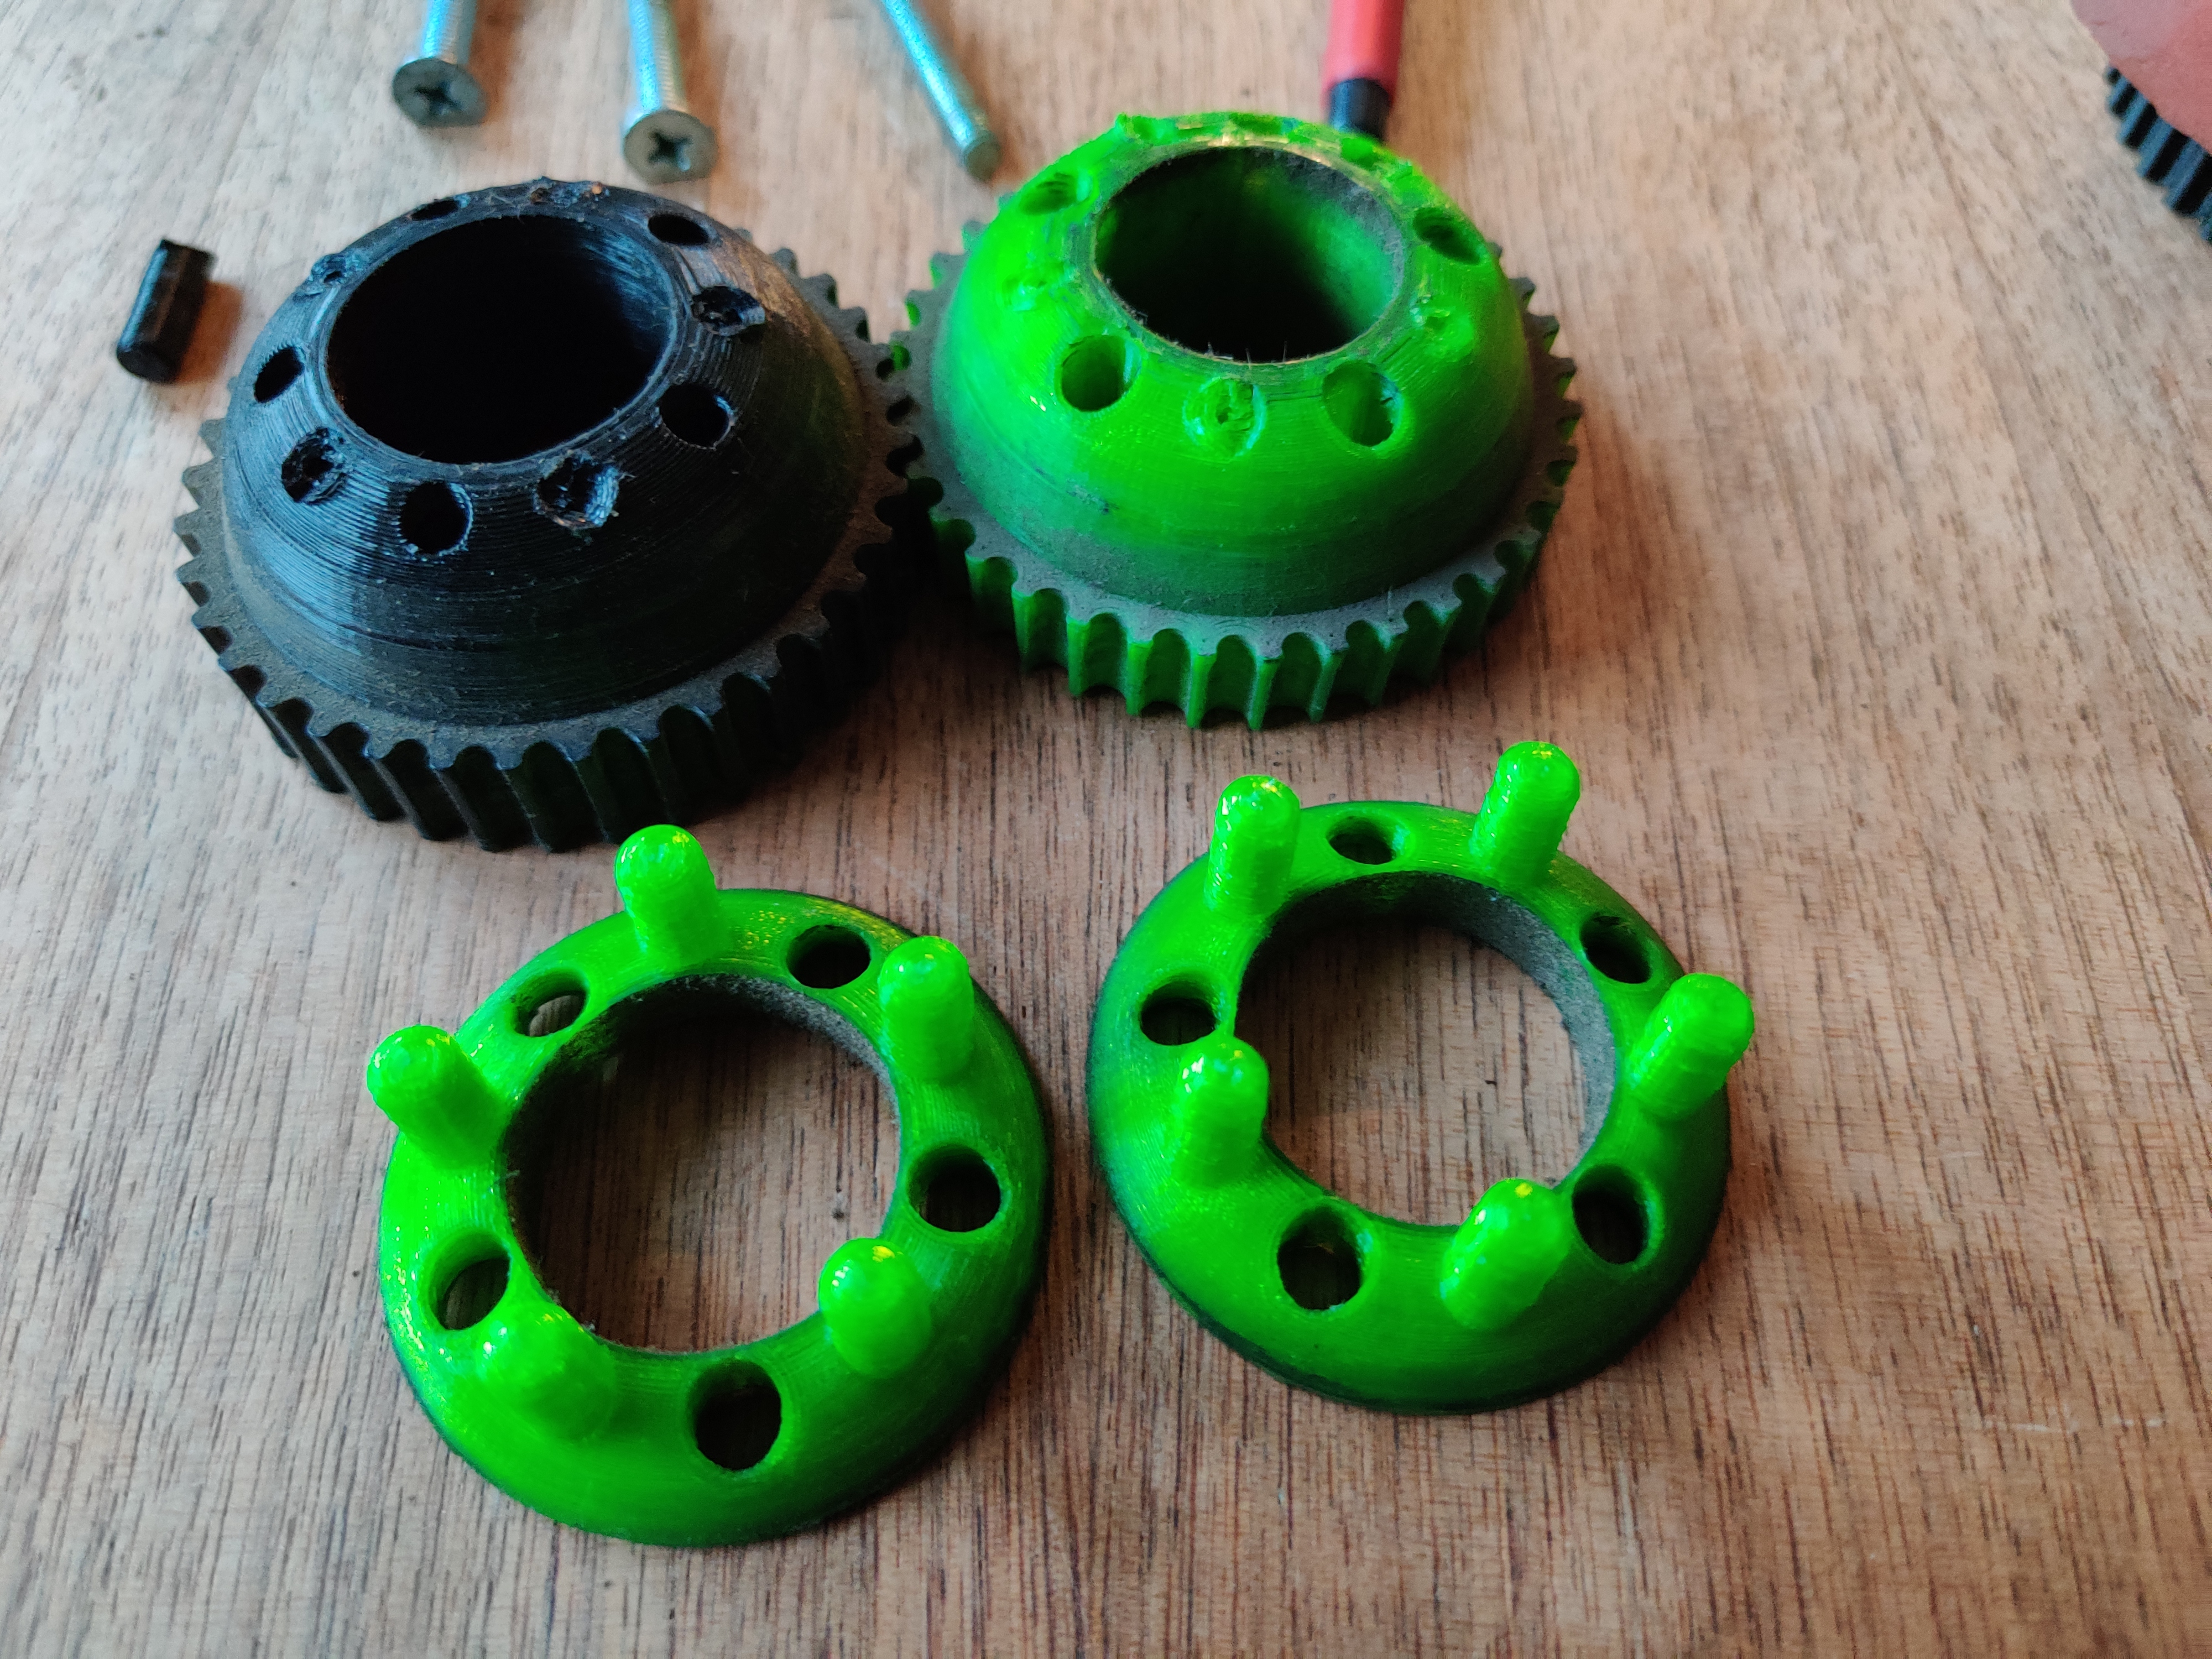
\includegraphics[width=.49\textwidth]{Footage/Pictures/Wheel pulley v1.jpg}
			}
			\caption[Vergleich der gedruckten Zahn- und Konterscheiben vor und nach mehreren Testfahrten]{(a) Die finale und zum Zeitpunkt des Verfassens dieses Dokumentes noch verbaute Version. (b) Der Zustand des ersten funktionalen Prototypes nach etwa~\qty{100}{\kilo\metre} Testfahrt. Neben zu erwartender Verschmutzung sei insbesondere auf das Fehlen der Führungsstifte zu achten. Das Zahnprofil und die Komponenten als ganze weisen darüber hinaus jedoch keinerlei Anzeichen von Materialversagen auf.}
			\label{fig:comparison printed parts used unused}
		\end{figure}


	\section{Kosten}\label{sec:cost}
		Das im Rahmen dieses Projektes gefertigte Antriebssystem lag mit \dEUR{264,75} gut unterhalb des fest gesetzten Preisrahmens von \dEUR{300}.
		Dies konnte allerdings nur realisiert werden, indem bereits vorhandene Aluminiumhalbzeuge und Schrauben genutzt und von einfachem und kostenfreiem Zugang zur FDM-Druck- und CNC-Fräsfertigung Gebrauch gemacht wurde.

		Externe Fertigung der Druckteile schlüge sich zwar mit \dEUR{23,03} und damit vergleichsweise geringen Kosten nieder, um unterhalb der Preisobergrenze zu bleiben war die Ersparnis der Fertigungs- und Materialkosten der Motorhalterung von \dEUR{170} jedoch maßgeblich.\par\medskip
		%
		Eine Aufstellung der Einzelkosten findet sich in \cref{tab:costs}.
		Die mit ``*'' gekennzeichneten Posten konnten im Rahmen des Projektes eingespart werden und sind mit Schätzwerten angegeben.
		Herstellung ohne Einsparmöglichkeit schlüge demnach mit \(\approx \dEUR{458,78}\) zu buche.
		\begin{table}[h]
			\caption[Kostenaufstellung der Einzelteile]{Kostenaufstellung der Einzelteile. Da nicht alle Teile gekauft werden mussten, sind, wo zutreffend, Schätzwerte angegeben und mit ``*'' gekennzeichnet.}%
			\label{tab:costs}
			\centering
			\begin{threeparttable}
				\begin{tabular}{lp{1cm}r}
					\toprule
					Teil											&& Kosten\\
					\midrule
					Druckteile\tnote{a}								&& *\dEUR{23,03}\\
					\hspace{5mm}Nur Material						&& \dEUR{0,86}\\
					Motorhalterungen\tnote{a}						&& *\dEUR{170}\\
					% \hspace{5mm}Nur Halbzeug						&& *\dEUR{17,67}\\
					Motoren											&& \dEUR{177}\\
					Schrauben										&& *\dEUR{3}\\
					Steckverbinder									&& \dEUR{2}\\
					Rollen\tnote{b}									&& \dEUR{34,75}\\
					Zahnriemen										&& \dEUR{29,4}\\
					Zahnriemenscheiben								&& \dEUR{19,6}\\
																	&&\\
					\textbf{Gesamt}									&& \dEUR{264,75}\\
																	&& *\dEUR{458,78}\\
					\bottomrule
				\end{tabular}
				\begin{tablenotes}\footnotesize
					\item[a]	Fertigungsangebot inklusive Material.
					\item[b]	Preis für zwei Rollen.
				\end{tablenotes}
			\end{threeparttable}
		\end{table}
% LTeX: language=de-DE
\chapter{Zusammenfassung}
	Die geforderte Maximalgeschwindigkeit konnte zwar im Leerlauf deutlich übertroffen werden, im Rahmen von Feldtests unterlag sie jedoch mit einem Spitzenwert von \qty{23,7}{\kilo\metre\per\hour} leicht den geforderten \qty{25}{\kilo\metre\per\hour}.
	Da sie jedoch softwareseitig limitiert wurde und bei Erreichen der gemessenen Maximalgeschwindigkeit noch ausreichend Leistungsreserven zur Verfügung standen ist davon auszugehen, dass, mit geeignetem Personenschutz höhere Geschwindigkeiten ohne weiteres erzielt werden können.

	Es ist zwar aus dem Stillstand heraus nicht möglich einen Hang hinauf zu beschleunigen, jedoch zeigte sich im Feld, dass bereits eine geringe Anfangsgeschwindigkeit etwa durch leichtes Anschieben ein Anfahren ermöglicht.
	So konnten Steigungen von bis zu \qty{7,5}{\percent} noch gut befahren werden, womit die Anforderungen an das Drehmoment übertroffen wurden.\par\medskip
	%
	Die Materialauswahl der mechanischen Komponenten kann für den Einsatzzweck als gut bezeichnet werden.
	Der bauartbedingte Spalt zwischen Motorflansch und Rotor lässt Eindringen von feinem Staub und Schmutz in das Innere der Motoren und damit an die Wicklungen und in die Spalte zwischen Magnete und Anker zu.
	Um ein frühzeitiges Versagen der Motoren zu verhindern, ist für zukünftige Revisionen ein Schutz in Form eines Schildes oder Ähnlichem zu empfehlen.
	Da der Riemen und die gedruckten Zahnriemenscheiben keine Spuren von lokalen Schäden aufweisen erscheint ein Riemenschutz zwar nicht zwingend erforderlich, mithin lagert sich um die Motorachse allerdings eine nicht unerhebliche Menge Schmutz an.
	Hier bieten sich die im vorgestellten Design bereits vorgesehenen Bohrungen für eine Abdeckung gut an.\par\medskip
	%
	Mit einem durchaus unhandlichen Gewicht des Gesamtsystems von \(\approx \qty{17,5}{\kilo\gram}\) ist anzuraten den Ladezustand im Blick zu halten.
	Händischer Transport über größere Strecken verbietet sich de facto und die hohe Masse erschwert manuelles Beschleunigen deutlich.
	Das Antriebssystem bietet nur bei den verwendeten Motoren --~auf Kosten von Leistung --~Einsparpotential bezüglich des Gewichtes.
	%
	Abschließend ist zu sagen, dass das Projekt trotz mangelnder Montagefreundlichkeit ein Erfolg war und --~es wird noch aktiv genutzt --~ist.
%-----------------------------------------------------------------
\newpage
\listoffigures
\listoftables
\appendix
\chapter{Anhang}
	% \begin{figure}[h]
	% 	\centering
	% 	\includesvg[width=\textwidth]{Assets/mosfets-Power MOSFETS}
	% 	\caption[Schaltplan der Leistungsendstufe des ESC]{Schaltplan der Leistungsendstufe des ESC\cite{vesc.documentation.2015}.}%
	% 	\label{fig:power mosfets}
	% \end{figure}
	% \newpage
	\begin{figure}[h]
		\centering
		\includegraphics[width=\textwidth]{Assets/ESC_Motor_Parameters.jpg}
		\caption[Testparameter, wie sie in der Konfigurationssoftware der ESC eingetragen wurden]{Testparameter, wie sie in der Konfigurationssoftware der ESC eingetragen wurden und gelten pro Motor. Einträge unter \texttt{Wattage} können ignoriert werden, da nicht verwendet.}%
		\label{fig:ESC motor params}
	\end{figure}
	\newpage
	\begin{figure}[h]
		\centering
		\includegraphics[width=\textwidth]{Assets/ESC_erpm.jpg}
		\caption[In-Software begrenzte elektrische Drehzahl]{In-Software begrenzte elektrische Drehzahl. Hier mit einem Wert von \qty{27850}{\per\minute}.}%
		\label{fig:ESC erpm setting}
	\end{figure}
	% \newpage
\printbibliography%
%=================================================================
\end{document}